%!TEX root = ../notas_de_clase.tex

\newpage
\section{Redes Neuronales}

\subsection{Introducción y arquitectura}

\subsubsection{Conceptos básicos}

Una red neuronal es un modelo de aprendizaje de máquinas inspirado en el funcionamiento de las neuronas en nuestro cerebro, sin embargo, a medida que se ha desarrollado la teoría en torno a las redes neuronales, este modelo se ha ido alejando progresivamente de su semejante biológico. Es más, investigadores argumentan que se debería dejar de lado el concepto de neurona puues es demasiado restrictivo en cuanto a los sistemas que podemos crear. 

Las redes neuronales son modelos computacionales basados en la conexión de múltiples unidades (neuronas) cuyo objetivo es aproximar una función $f^{*}$, más específicamente, definir un mapping $y = f(x;\theta)$ aprendiendo los parámetros $\theta$ que resultan en la mejor aproximación posible. Su gran ventaja radica en la posiblidad de entrenarlas con datos crudos, es decir, no es necesario extraer características relevantes de la data y en vez, se permite que el algoritmo aprenda cuales son. 

Los modelos escenciales de redes nueronales se conocen como \textbf{feedforward neural networks}, o \textbf{multilayer perceptrons} (MLPs) y se conocen como redes ya que son típicamente el resultado de composiciones sucesivas de varios tipos de funciones $f^{(1)},f^{(2)},f^{(3)}, \dots f^{(l)} .$, se dice que $f^{(i)}$ es la i-ésima capa de la red, mientras que $l$, la cantidad de capas, se le conoce como \textbf{profundidad}. Las capas intermedias se les conocen como \textbf{capas ocultas} y el uso de redes neuronales con una múltiples capas se le conoce como \textbf{deep learning}, aunque este término se usa para problemas más específicos de aprendizaje de máquinas usando redes neuronales profunidas (ver sección 3.5).

\begin{figure}[H]
	\captionsetup{font=small,labelfont=small}
	\caption{Ejemplo de una red neuronal de 1 capa: (\textit{izquierda}) Se muestra la red con inputs $x_1$ y $x_2$, que luego pasan a la capa oculta para producir el output $y$. (\textit{derecha}) Misma red con una representaci\'on vectorial de las capas. La matriz ${\bm{W}}$ describe el mapping de ${\bm{x}}$ a ${\bm{h}}$, y la matriz $w$ el mapping de ${\bm{h}}$ a $y$.}
	\centering
	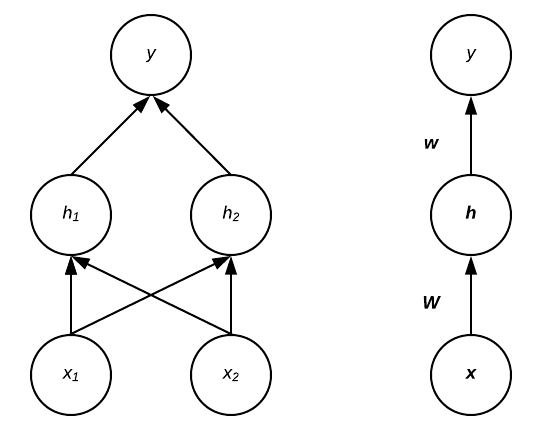
\includegraphics[scale=.5]{img/cap7_F1NN1L.png}
\end{figure}

Como se puede apreciar en la figura, los coeficientes ${\bm{W}}$ y $w$ se usan para producir el output para la siguiente capa (denominados \textbf{pesos}), por lo que la primera operaci\'on de esta red ser\'a entregar $h_{1}$ y $h_{2}$ mediante la transformaci\'on ${\bm{W}^{T}}\bm{x} + \bm{b}^{(1)}$. Luego, esta red aplica $w^{T} \boldsymbol{h} + b^{(2)}$ para producir el output $y$. Los coeficientes $\bm{b}^{(1)}$ y  $b^{(2)}$ se conocen como t\'erminos de \textbf{bias} (sesgo). Todos los parámetros de la red neuronal, los pesos y \textit{bias}, serán agrupados en el t\'ermino $\bm{\theta}$.


\subsubsection{El perceptrón y funciones de activación}

El \textit{perceptrón} corresponde a la forma más básica de una red neuronal, esta recibe un input numérico $x = (x_i)_{i=1}^n \in \R^n$ y computa la suma ponderada $u = x_1w_1 + x_2w_2 + \dots + w_nx_n + b$ donde $W = (w_i)_{i=1}^n \in \R^n$ corresponden a los \textbf{pesos} (weights) y $b \in \R$ el \textbf{sesgo} (bias). 
A continuación, se aplica una función de activación $f$ y se entrega un output $h = f(u)$.  
\begin{figure}[H]
  \centering
  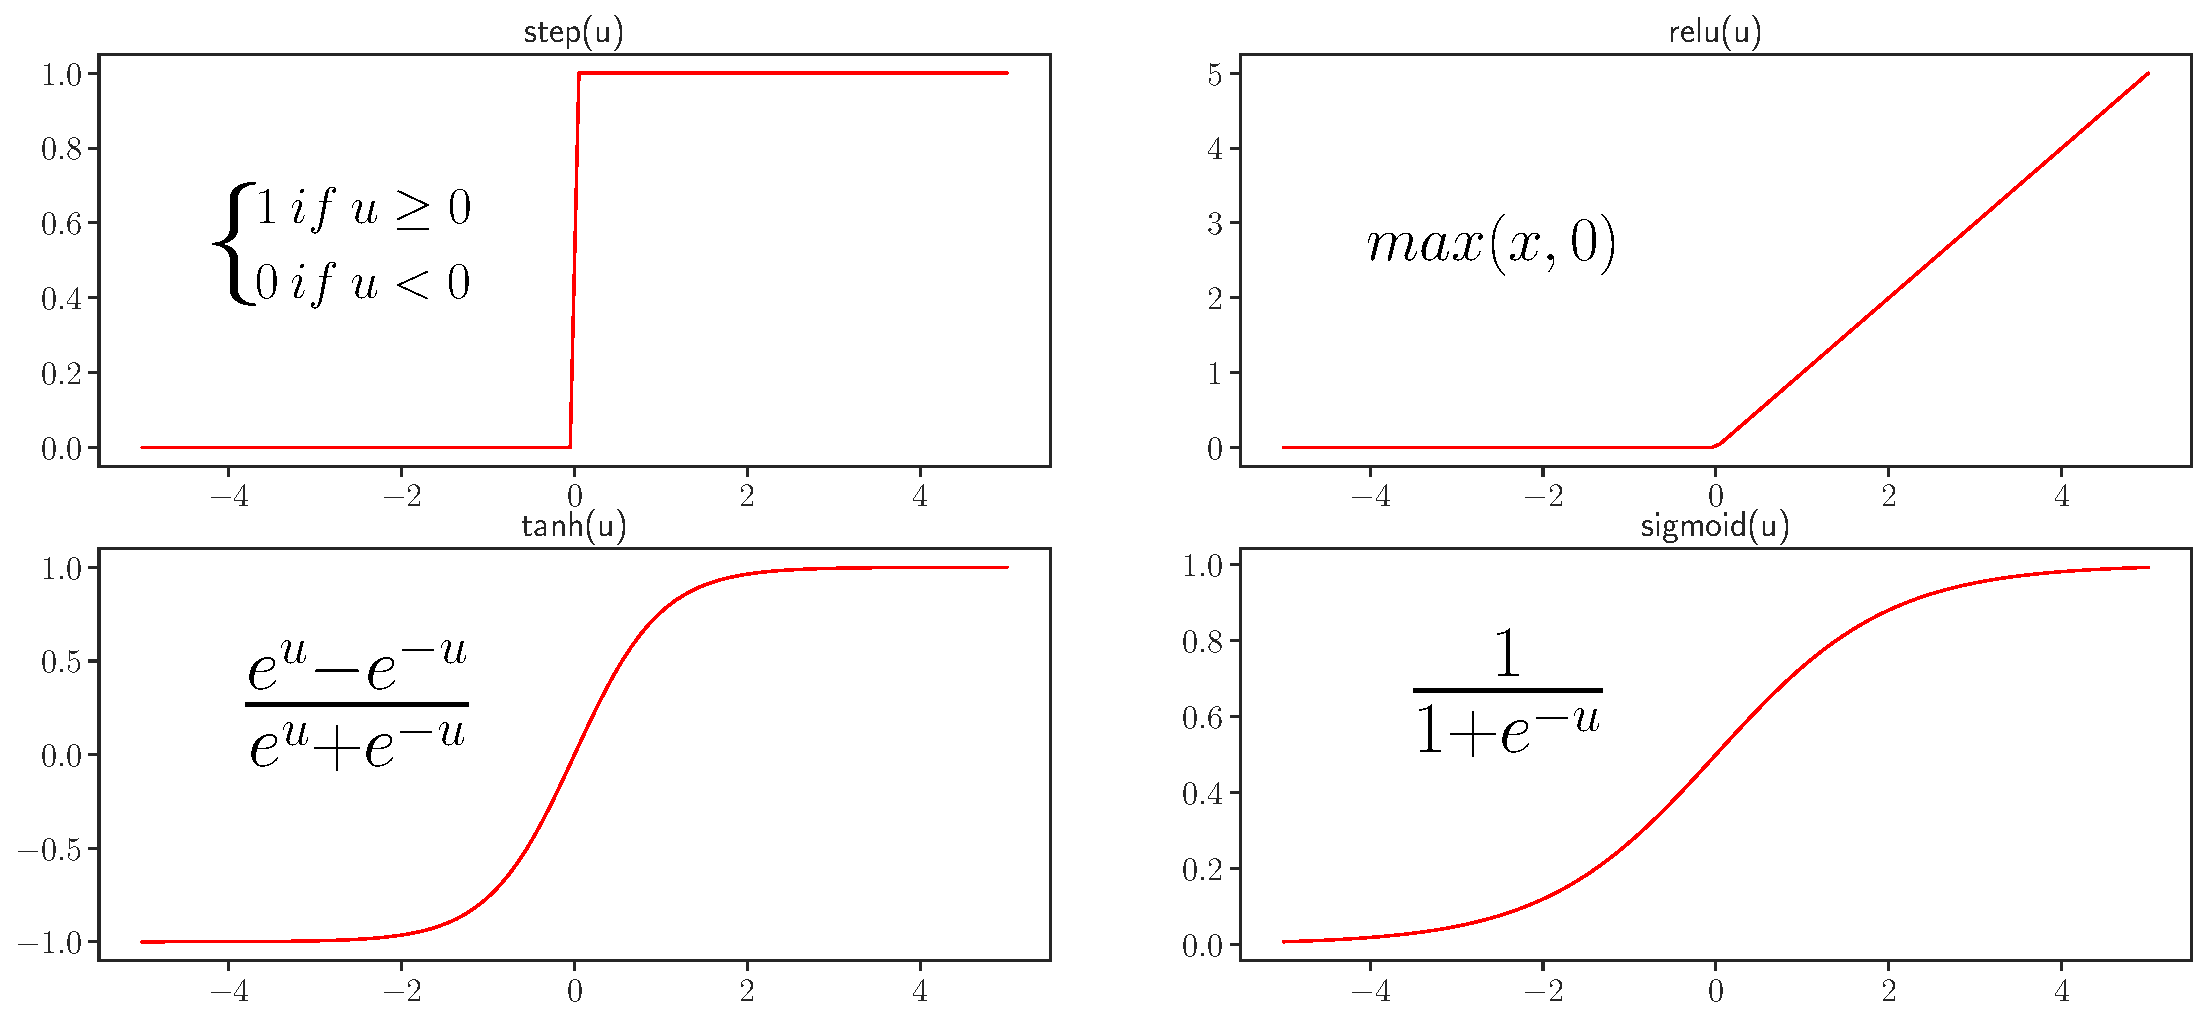
\includegraphics[scale=.3]{img/cap5_activaciones}
  \caption{Algunos ejemplos de funciones de activación}
\end{figure}

Un conjunto de perceptrones interconectados forman las capas de la red (de ahí el nombre multilayer perceptrons), las funciones de activación son en general transformaciones no lineales que buscan dar la flexibilidad necesaria al modelo para aprender funciones extremadamente complejas, lo anterior se sustenta en el siguiente teorema 


\begin{theorem}[UAT - Ancho arbitrario (Horniket al., 1989; Cybenko, 1989)]

	Sea $f^{*}$ una función objetivo Borel Medible (por ejemplo $f^{*}:[0,1]^k \rightarrow [0,1]$ continua con $k \in \N$) y sea $f$ una función de activación no polinomial acotada, entonces para todo $\epsilon > 0$ existen $W,b$ definidas como antes y $U$ la matriz de pesos de la última capa tales que 
	\[
	F(x) = f(xW+b)U, \quad 
	|F(x)-f^{*}(x)|<\epsilon \quad \forall x \in Dom(f^{*}) 
	\]
\end{theorem} 

Es decir, para una red de una sola capa escondida con la suficiente cantidad de perceptrones, es posible aproximar una función objetivo razonable tan finamente como se desee. Notar que lo anterior es un resultado que considera el ancho (cantidad de perceptrones en la capa) y que este podría ser arbitrariamente grande además, la red podría tener una baja capacidad de generalización dependiendo de la complejidad de los datos con los que se pretende trabajar. Es por esto que surge la necesidad de arquitecturas más complejas, es decir, con mayor cantidad de capas (mayor profundidad) pero menor cantidad de perceptrones y por suerte, UAT para profunidad arbitraria también es valido. 

Veamos el siguiente ejemplo: 

\begin{figure}[H]
    \centering
    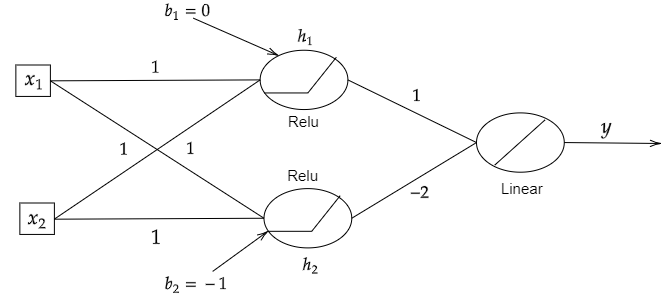
\includegraphics[scale=.5]{img/cap7_xor}
    \caption{Red Neuronal de 2 perceptrones para XOR}
\end{figure}

En su forma matricial 
$$
(h_1 , h_2) = \text{Relu} \left ( \begin{pmatrix}
x_1 & x_2  
\end{pmatrix} \begin{pmatrix}
1 &1 \\ 
 1 & 1
\end{pmatrix} + \begin{pmatrix}
0 & -1 
\end{pmatrix}\right) \hspace{0.5cm} h = \text{Relu}(xW + b)
$$

$$
y = \begin{pmatrix}
h_1 & h_2 
\end{pmatrix}\begin{pmatrix}
1 \\ 
-2 
\end{pmatrix} + (0) \hspace{0.5cm} y = hU + c
$$
Donde $U$ y $c$ corresponden al peso y bias de la última capa respectivamente, es una red capaz de computar el operador XOR.

%\begin{tabular}{| c  c | c |}
%    \hline
%    $x_1$ & $x_2$ & $y$ \\ \hline
%    0 & 0 & 0 \\
%    1 & 0 & 1 \\
%    0 & 1 & 1 \\ 
%    1 & 1 & 0 \\ \hline
%\end{tabular}. 

\subsubsection{Arquitectura de una red neuronal}

Como vimos anteriormente, no basta con una red arbitrariamente ancha para lograr el objetivo de aproximar $f^{*}$ con una alta capacidad de generalización, la \textbf{arquitectura} de una red neuronal se refiere a la totalidad de su estructura, es decir, la cantidad de capas, perceptrones por capa, conexión entre unidades, funciones de activación, etc... 

\begin{figure}[H]
	\centering
	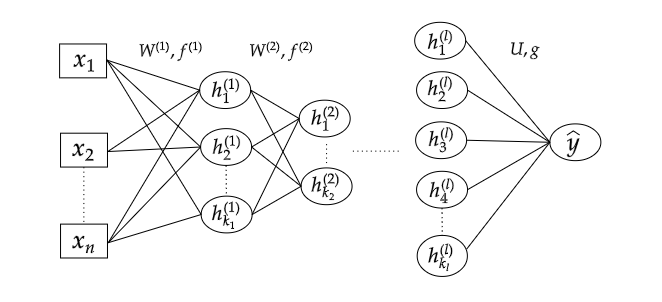
\includegraphics[scale=.5]{img/cap7_red}
	\caption{Una red con mayor profundidad}
\end{figure}

Vamos a utilizar la siguiente notación a partir de este punto 

\begin{equation}
	h^{(k)} = f^{(k)}(h^{(k-1)}W^{(k)} + b^{(k)}) \hspace{0.3cm} \forall k \in \{1 ,\dots, l\}, \quad h^{(0)}=x
	\end{equation}
	\begin{equation}
	\hat{y} = g(h^{(l)}U + c)
\end{equation}
	
Donde $g$ es la función aplicada en la capa de output y es la que define la $\textbf{unidad de output}.$

\subsubsection{Función de costos y unidades de output}

Una de las principales diferencias entre los modelos lineales antes vistos y una red neuronal, es que el uso de ciertas funciones de activaci\'on hacen que la funci\'on de costos no sea convexa, esto hace que el entrenamiento realizado en base a descenso de gradiente no entregue garant\'ias de que se alcanzar\'a el \'optimo global, o una buena solución en términos generales, ya que el algoritmo podría estancarse en un optimo local que entregue resultados pobres. 

En la mayor\'ia de los casos, el modelo param\'etrico define una distribuci\'on $p(y|\bm{x}; \bm{\theta})$, por lo que los par\'ametros del modelo se estimar\'an usando m\'axima verosimilitud, as\'i, se optimizar\'a la log-verosimilitud negativa, es decir, la \textbf{funci\'on de costos} a usar ser\'a la \textbf{cross-entropy}:

\begin{equation}
J(\bm{\theta}) = -\E_{\bm{x},\bm{y}\sim \hat{p}_{\textrm{data}}}(\textrm{log}\; p_{\textrm{modelo}}(\bm{y}|\bm{x}))
\end{equation}

De esta forma la elecci\'on de la \textbf{unidad de output} definir\'a la forma que toma la funci\'on de costos, pero no ser\'a necesario definir una funci\'on especifica para cada problema; en general siempre se resolver\'a el problema por m\'axima verosimilitud. La elecci\'on en la unidad de output depender\'a del tipo de problema que se quiera resolver, por ejemplo

\begin{enumerate}
  \item Unidad de output lineal $\hat{\bm{y}} = h^{(l)}U + c$ 

  Útil para cuando se busca retornar la media de una distribución Gaussiana condicional $p(\bm{y}|\bm{x}) = \mathcal{N}(\bm{y}|\hat{\bm{y}};\bm{I})$, el problema de maximizar la log-verosimilitud será equivalente a minimizar el error cuadrático medio por lo que resulta adecuado para un problema de regresión.

  \item Unidad de output sigmoidal $\hat{{y}} = \text{sig}(h^{(l)}U + c)$ 

  Este se utiliza para problemas de clasificación binaria, para resolver el problema de máxima verosimilitud, se modela utilizando una distribución Bernoulli en $y$ condicional en $x$. La unidad de output modela entonces $P(y=1|\bm{x})$ o la probabilidad de pertenecer a la clase 1.
   

  \item Unidad de output softmax $\hat{{y}} = \text{softmax}(h^{(l)}U + c)$  

  Es una generalización de la función sigmoidal definida como 
  \begin{equation*}
  \text{softmax}(z)_i = \frac{e^{z_i}}{\sum_{j}e^{z_j}}
  \end{equation*}
  y se utiliza para el caso de clasificación multiclase. 
  %Se podrían agregar propiedades como estabilidad numérica producto de invarianza a la adición 
\end{enumerate}


\subsection{Entrenamiento de una red neuronal}

\subsubsection{Forward Propagation}

Al usar una red neuronal \textit{feedforward}, la información fluye a través de la red desde el ingreso de un input $x$ hasta producir un output $\hat{y}$. Esto se conoce como \textbf{forward propagation} y es la que durante el entrenamiento calcula el costo $J(X, \theta)$ 
El algoritmo que la describe es el siguiente:

\begin{algorithm}[H] % H = forzar está posición 
	\caption{Forward Propagation}\label{ML:Algorithm1}
	\textbf{Requerir}: Profundidad de la red, $l$ \\
	\textbf{Requerir}: $\bm{W}^{(k)}, k \in \{1,...,l\}$, pesos de la red \\
	\textbf{Requerir}: $\bm{b}^{(k)}, k \in \{1,...,l\}$, parámetros bias de la red \\
	\textbf{Requerir}: $\bm{x}$, el input \\
	\textbf{Requerir}: $U,c,g$, matriz de peso, bias y función de output de la última capa respectivamente 
	\begin{algorithmic}[1]
		\State $\bm{h}^{(0)} \gets \bm{x}$
		\For{$\;k = 1,...,l$:}
			\State $\bm{u}^{(k)} \gets  \bm{h}^{(k-1)}\bm{W}^{(k)} + \bm{b}^{(k)}$
			\State $\bm{h}^{(k)} \gets f^{(k)}(\bm{u}^{(k)})$
		\EndFor
		\State $\bm{\hat{y}} \gets g(\bm{h}^{(l)}U+c)$
		\State $J \gets L(\bm{\hat{y}},\bm{y})$
	\end{algorithmic}

\end{algorithm}


\subsubsection{Backward Propagation - Preliminares}

El algoritmo de $\textbf{backpropagation}$ permite que la información del costo fluya en sentido inverso a través de la red para calcular el gradiente de manera computacionalmente eficiente. 

El gradiente se calculará de esta forma ya que, aunque es posible obtener una expresión analítica para este, evaluar la expresión puede ser muy caro computacionalmente. 

Luego de obtener el gradiente, otro algoritmo como descenso de gradiente estocástico realizará el aprendizaje usando la expresión que fue calculada. 

El algoritmo de backpropagation ha experimentatdo un resurgimiento en estas últimas décadas por su implementación en redes neuronales para tareas tales como reconocimiento de imágenes o procesamiento de lenguaje natural. 
Es considerado un algoritmo eficiente e implementaciones modernas de estas aprovechan el paralelismo de las GPU para mejorar su rendimiento. 

Antes de comenzar a describir el algoritmo, debemos tener en cuenta que.   
\begin{itemize}

	\item Utilizaremos la notación para el paso intermedio antes de aplicar la función de activación como $u = hW + b$
  
	\item Es recurrente que en la etapa de entrenamiento de la red el conjunto de datos se entreguen en pequeños paquetes (\textbf{mini-batch}), es decir $(x^d)_{d=1}^N$  conjunto de $N$ inputs, luego $u_{dj}^{(k)}$ corresponde al valor de $u$ para el input $d$ en el nodo $j$ para la capa $k$. Todo esto con el fin de aprovechar lo más posible la optimización en operaciones de matrices que ofrecen las GPU.

   
   \item Haremos la deducción del algoritmo de backpropagation para una función de error MSE en un problema de regresión.
   \[
	J(X ,\theta) = \frac{1}{2N}\sum_{d=1}^N(\hat{y}_d-y_d)^2
	\]	
  
\end{itemize} 

Nuestro objetivo será actualizar todos los valores $w_{ij}^{(k)}$ (peso del nodo $i$ al nodo $j$ en la capa $k$). Es decir, para utilizar el método del descenso de gradiente es necesario calcular $\frac{\partial J(X , \theta) }{\partial w_{ij}^{(k)}}$ notemos que 
\[
\frac{\partial J(X , \theta) }{\partial w_{ij}^{(k)}} = \frac{1}{N}\sum_{d=1}^N \frac{\partial}{\partial w_{ij}^{(k)}} \left ( \frac{1}{2}(\hat{y}_d-y_d)^2 \right) = \frac{1}{N}\sum_{i=1}^N \frac{\partial J_d}{\partial w_{ij}^{(k)}}
\]

Utilizando la regla de la cadena 
\[
\frac{\partial J_d}{\partial w_{ij}^{(k)}} = \frac{\partial J_d}{\partial u_{dj}^{(k)}}\frac{\partial u_{dj}^{(k)}}{\partial w_{ij}^{(k)}}
\] 
La expresión $\frac{\partial J_d}{\partial u_{dj}^{(k)}}$ corresponde a un término de \textbf{error} y lo denotaremos \
\[
\delta_{dj}^{(k)} \equiv \frac{\partial J_d}{\partial u_{dj}^{(k)}}
\] 
Mientras que para el otro término tenemos que 
\[
\frac{\partial u_{dj}^{(k)}}{\partial w_{ij}^{(k)}} = \frac{\partial}{\partial w_{ij}^{(k)}} \left ( \sum_{a = 1}^{k_k}w_{aj}^{(k)}h_{da}^{(k-1)} + b_j^{(k)} \right) = h_{di}^{(k-1)}
\] 
y así 
\[
\frac{\partial J_d}{\partial w_{ij}^{(k)}} = \delta_{dj}^{(k)}  h_{di}^{(k-1)}
\]
El gradiente total, será la suma de los $N$ gradientes y que expresaremos en su forma matricial
\begin{equation}
\frac{\partial J}{\partial w_{ij}^{(k)}} = \sum_{d=1}^N \delta_{dj}^{(k)}  h_{di}^{(k-1)}  \Rightarrow  \frac{\partial J}{\partial W^{(k)}} = (h^{(k-1)})^T @ \hspace{0.1cm} \delta^{(k)}
\end{equation}
Omitiremos la constante $1/N$ hasta el final del algoritmo.




\subsubsection{Backward Propagation - Capas ocultas}

Nuevamente, de la regla de la cadena
\[
\delta_{dj}^{(k)} = \frac{\partial J_d}{\partial u_{dj}^{(k)}} = \sum_{a=1}^{k_{k+1}} \frac{\partial J_d}{\partial u_{da}^{(k+1)}} \frac{\partial u_{da}^{(k+1)}}{\partial u_{dj}^{(k)}} = \sum_{a=1}^{k_{k+1}} \delta_{da}^{(k+1)} \frac{\partial u_{da}^{(k+1)}}{\partial u_{dj}^{(k)}}
\] 

no es difícil ver que

\[
\frac{\partial u_{da}^{(k+1)}}{\partial u_{dj}^{(k)}} = w_{ja}^{(k+1)}f'(u_{dj}^{(k)})  \Rightarrow  \delta_{dj}^{(k)} = f'(u_{dj}^{(k)})\sum_{a=1}^{k_{k+1}}w_{ja}^{(k+1)}\delta_{da}^{(k+1)}
\]

Hemos encontrado una expresión para calcular el gradiente en una capa $k$ en base al gradiente de la siguiente capa $k+1$ (De aquí el nombre \textbf{backward propagation}).
\newline 

Lo anterior en su forma matricial queda descrito por
\begin{equation}
\delta^{(k)} = f'(u^{(k)}) * \left ( \delta^{(k+1)} @ \hspace{0.1cm} (W^{(k+1)})^T \right )
\end{equation}
Lo único que queda para presentar el algoritmo final es calcular los gradientes en la última capa (output)


\subsubsection{Backward Propagation - Capa de output}

Estamos suponiendo un problema de regresión por lo que el output será de una sola salida y la función de error es MSE, entonces 
\[
\delta_{d1}^{(l)} = \frac{\partial J_d}{\partial u_{d1}^{(l)}} = (\hat{y}_d-y_d) (\hat{y}_d)' 
\] 
Además, la función de activación en el output será lineal y por tanto $(\hat{y}_d)' = 1$, finalmente el término de normalización $N$ se agrega en este paso.  La forma matricial queda en 
\begin{equation}
\label{eq:capa_output}
\delta^{(l)} = \frac{1}{N}(\hat{y}-y) 
\end{equation}

Además de lo anterior, se puede probar también que 
\begin{equation}
	\frac{\partial J}{\partial b^{(k)}} = \text{Sum}_1 \left ( \delta^{(k)} \right ), \quad \frac{\partial J}{\partial U} = (h^{(l)})^T @ \delta^{(l)}, \quad \frac{\partial J}{\partial c} = \text{Sum}_1 \left ( \delta^{(l)}\right )
\end{equation}

Donde $\text{Sum}_1$ es la suma sobre la primera dimensión de la matriz, es decir  $\text{Sum}_1(A) = (\sum_{i}A_{ij})_j$. Con todo lo anterior ya estamos en condiciones de mostrar el algoritmo de backpropagation.

\begin{algorithm}[H]
	\caption{Backward Propagation} \label{ML:Algorithm2}
	\textbf{Requerir: } learning rate $\lambda$ para descenso de gradiente estocástico
	\begin{algorithmic}[1]
	\State Forward propagation, guardar  ($\hat{y})$ , $(u^{(k)})$ y $(h^{(k)})$.
	\State Evaluar el error de la última capa $\delta_1^{(l)}$  según la unidad de output
	\State  Actualizar $U \gets U - \lambda \frac{\partial J}{\partial U}$
	\State Actualizar $c \gets c - \lambda \frac{\partial J}{\partial c}$
	\For{$k = l-1,...,1$:}
		
		\State Calcular $\delta^{(k)}$ con las ecuaciones en las capas ocultas
		\State Evaluar las derivadas parciales $\frac{\partial J}{\partial W^{(k)}}$ y $\frac{\partial J}{\partial b^{(k)}}$
		\State Actualizar $W^{(k)} \gets W^{(k)} - \lambda \frac{\partial J}{\partial W^{(k)}}$
		\State Actualizar $b^{(k)} \gets b^{(k)} - \lambda \frac{\partial J}{\partial b^{(k)}}, \quad$
		
	\EndFor

	\end{algorithmic}
	
\end{algorithm}

\begin{remark}
	El algoritmo anterior debe ser aplicado para todos los batch del conjunto de entrenamiento, la cantidad de veces que se pase por todos los datos de entrenamiento, se conoce como \textbf{épocas}, en general un mayor número de épocas disminuye el error de entrenamiento, sin embargo, muchas épocas podrían reducir la capacidad de generalización debido al \textbf{overfitting}.	
\end{remark}

\subsection{Regularización}

Las redes neuronales y algoritmos de deep learning son aplicados a tareas extremadamente complejas como lo son el procesamiento de im\'agenes, audio, y texto. Controlar la complejidad de un modelo no solo se reduce a encontrar el tamaño y cantidad de parámetros adecuados, como se ha visto para otros modelos de aprendizaje de m\'aquinas, sino que en la pr\'actica el modelo con el mejor ajuste por lo general ser\'a un modelo grande (profundo) que ha sido regularizado apropiadamente. 

El objetivo de las técnicas de regularización es el de reducir el \textit{error de generalización}, es decir, el error esperado al clasificar datos nunca antes vistos pero manteniendo la capacidad del modelo (profundidad, cantidad de nodos, funciones de activación, etc...)

\subsubsection{Regularización ${L}^{2}$}

Una regularizaci\'on que se basa en limitar la norma de los parámetros del modelo es la ya conocida \textbf{regularizaci\'on} $\bm{L}^{2}$ (o \textbf{ridge regression}), mediante la cual se obtiene la funci\'on objetivo regularizada $\tilde{J}$:

\begin{equation}
\tilde{J}(\bm{\theta};\bm{X},\bm{y}) = J(\bm{\theta};\bm{X},\bm{y}) + \frac{\alpha}{2}||\bm{\theta}||^{2}_{2}
\end{equation}

en donde el hiperpar\'ametro $\alpha \in [0,\infty[\ $ indica qué tanta importancia se le da al termino de regularización sobre el objetivo, no habrá regularizaci\'on cuando $\alpha = 0$ y se observará un mayor efecto regularizador a medida que $\alpha$ crece. Cabe destacar que t\'ipicamente en una regularizaci\'on por la norma solo se regularizan los \textit{pesos}, dejando los t\'erminos de \textit{bias} sin regularizar. Esto ya que cada t\'ermino de \textit{bias} controla el comportamiento de solo una variable implicando que no se introduce mucha varianza al dejarlos sin regularizar, por otro lado, regularizar los \textit{bias} puede inducir un alto nivel de \textit{underfitting}.

No es dificil ver que esta regularización es equivalente a la actualización de parámetros según gradiente estocástico de la forma 

\begin{equation*}
W^{(k)} \gets (1-\beta) W^{(k)} - \lambda \frac{\partial J}{\partial W^{(k)}}, \quad \beta = \lambda \alpha
\end{equation*}
y por eso también es llamada \textit{weight decay} y es la forma en que se implementa en la práctica. 

\subsubsection{Dropout}

\textbf{Bagging} consiste en entrenar m\'ultiples modelos y evaluarlos en cada dato del set de testeo. Esto no es pr\'actico para redes neuronales, ya que un solo modelo puede ser muy caro de entrenar y evaluar. \textbf{Dropout} provee una aproximaci\'on barata (computacionalmente) para entrenar y evaluar \textit{bagged} ensambles compuestos por una cantidad exponencial de redes neuronales.

Esta técnica de regularización consiste en entrenar en cada iteración una fracción de los pesos mediante una elección aleatoria. Su implementación es bastante simple y basta con definir para cada capa $k$ la probabilidad $1-p_k$ de 'apagar' una neurona en particular. Esto corresponde a la aplicación de una máscara binaria $M^{(k)}$ de la siguiente forma:

\begin{equation}
h^{(k)} = f^{(k)}(h^{(k-1)}W^{(k)} + b^{(k)}) *  \frac{M^{(k)}}{p_k}, \quad M^{(k)}_i \sim \text{Bernoulli}(p_k) \hspace{0.2cm} \forall i,k
\end{equation}

\begin{figure}[H]
	\captionsetup{font=small,labelfont=small}
	\caption{Dropout entrena potencialemente todas las subredes que se puedan formar a partir de la red neuronal original (primer recuadro) al apagar el output que producen las distintas unidades}
	\centering
	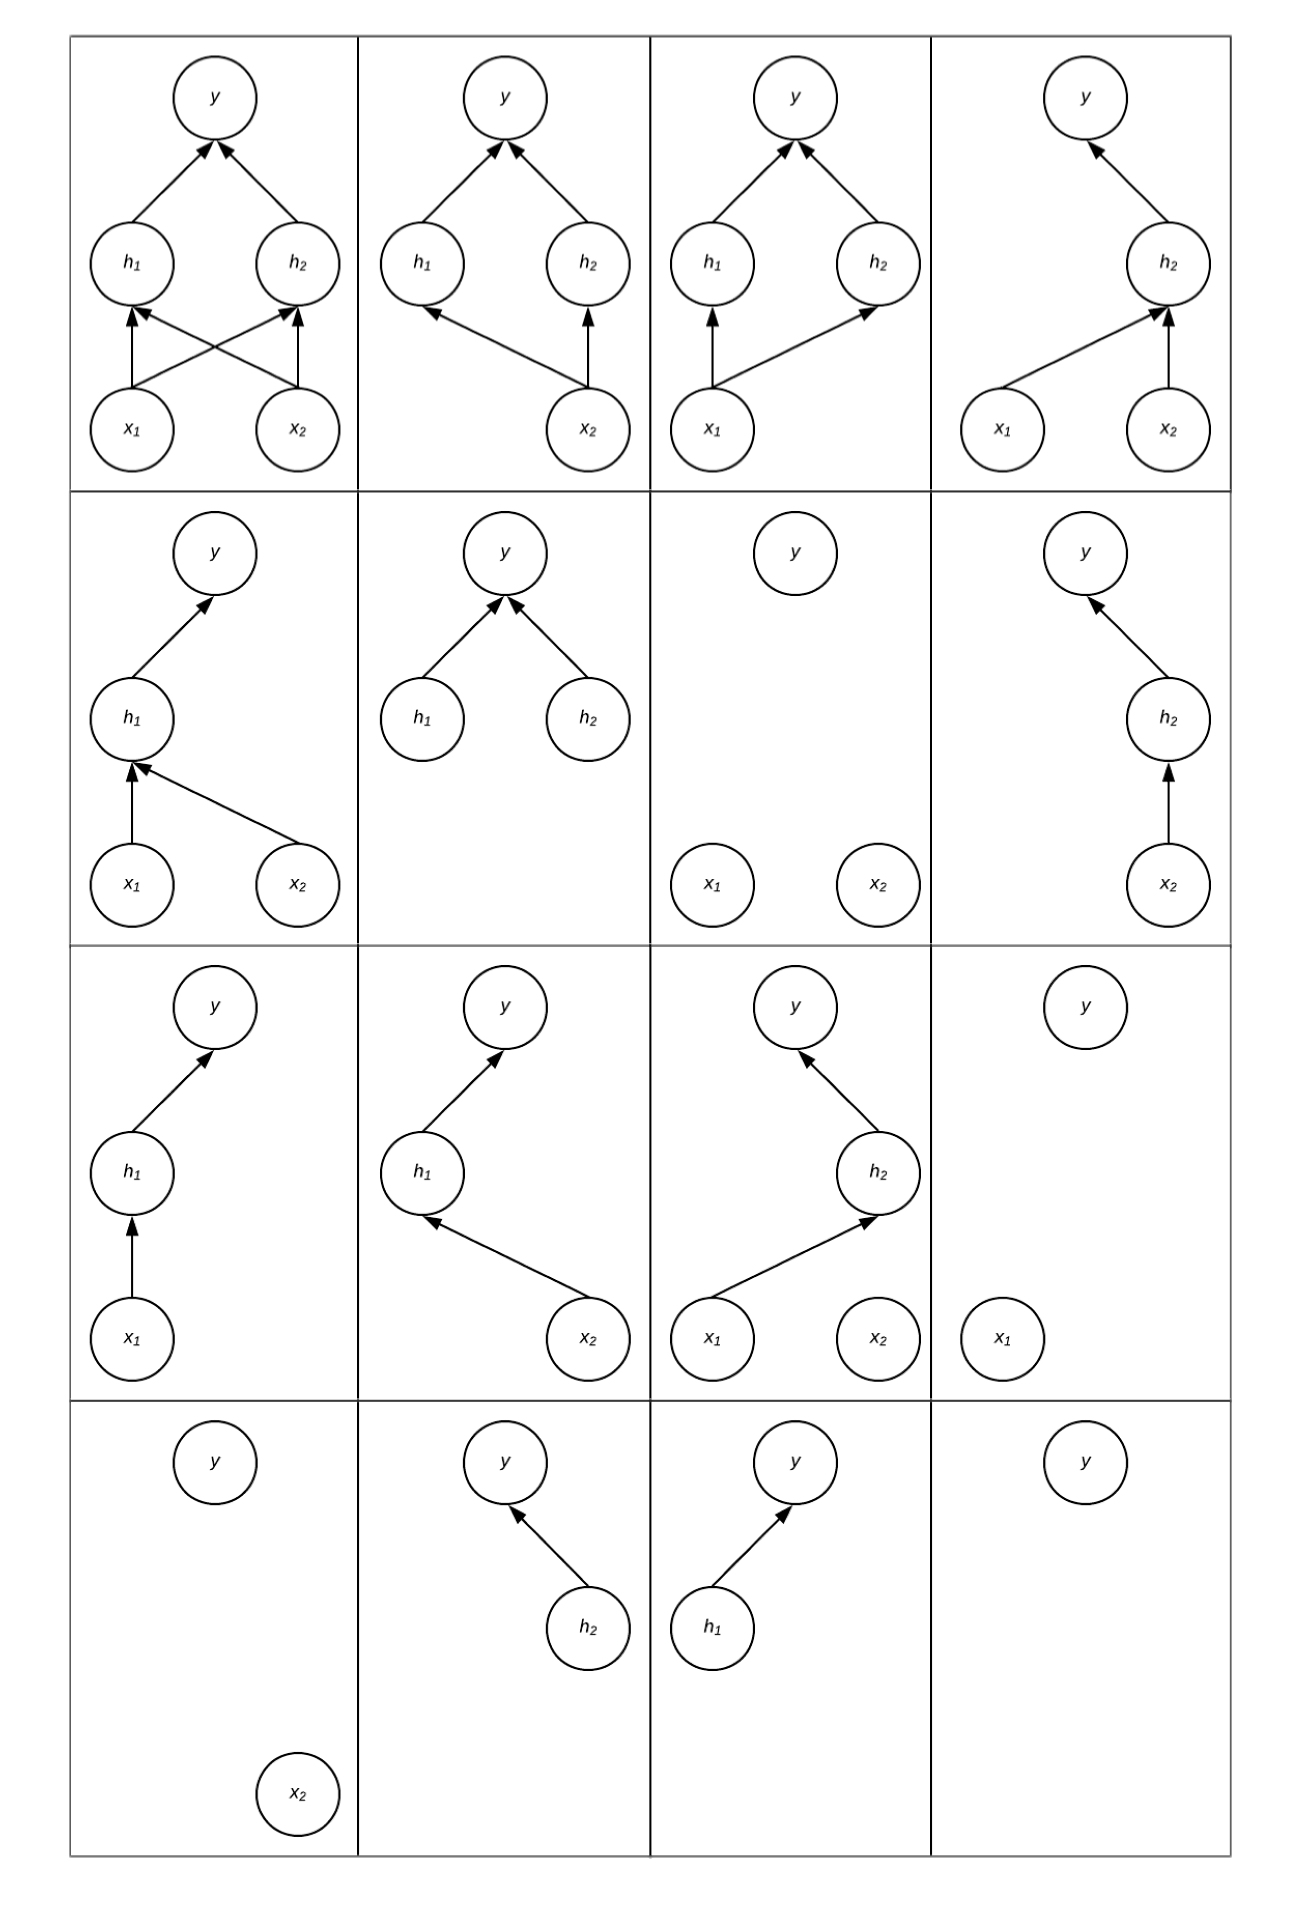
\includegraphics[scale=.25]{img/cap7_Dropout.png}
\end{figure}

Notar que al aplicar el algoritmo de backpropagation, también es necesario 'apagar' las neuronas que no participaron del forward para evitar que sean entrenadas. 

\subsubsection{Otros m\'etodos de regularizaci\'on}

Otras formas de regularizaci\'on tambi\'en buscan 
introducir alguna fuente de ruido (como en dropout) para que la red neuronal aprenda principalmente los par\'ametros m\'as importantes, as\'i logrando un bajo error de generalizaci\'on. Una de estas t\'ecnicas es \textbf{dataset augmentation}, que consiste en generar nuevos datos de entrenamiento (inyectando ruido en el set de entrenamiento), creando datos $\bm{x}$ falsos para los cuales se pueda tener una etiqueta $y$ (por ejemplo, una imagen invertida de un gato sigue siendo un gato), o \textbf{entrenamiento adversarial}, en donde se perturban ejemplos para fortalecer a la red (por ejemplo, cambiar pixeles de una imagen que generen cambios imperceptibles para un humano pero que pueden afectar fuertemente la capacidad de predicci\'on de un modelo). Otra t\'ecnica es \textbf{noise injection} en los pesos (Jim et al., 1996; Graves, 2011), lo cual se puede interpretar como una implementaci\'on estoc\'astica de inferencia Bayesiana sobre los pesos, debido a que el aprendizaje considerar\'ia que los pesos son inciertos y, por lo tanto, representables mediante una distribuci\'on de probabilidad.

Tambi\'en, por supuesto, \textbf{early stopping} es una t\'ecnica v\'alida para regularizar redes neuronales al detener el entrenamiento cuando el error de generalización en el conjunto de validación comience a aumentar.  

\subsection{Algoritmos de optimización}

Como ya se ha comentado, la optimizaci\'on en redes neuronales busca resolver un problema particular: encontrar los par\'ametros $\bm{\theta}$ que disminuyan significativamente $J(\bm{\theta})$, que depende de alguna medida de desempe{\~{n}}o evaluada en la totalidad del set de entrenamiento, luego se evaluá el error en el set de validaci\'on para tener una idea del desempeño, finalmente se ven los resultados en el set de testeo. 

Esto se reduce a minimizar la esperanza del error sobre la distribuci\'on generadora de los datos, $p_{\textrm{data}}$:

%[ posiblemente minimizando mediante hiperpar\'ametros tambi\'en una funci\'on de costos regularizada $\tilde{J}(\bm{\theta})$ ]

\begin{equation}
J^{*}(\bm{\theta}) = \E_{(\bm{x},y)\sim {p}_{\textrm{data}}}L(f(\bm{x};\bm{\theta}),y)
\label{gradiente_completo}
\end{equation}

Reemplazamos la expresión anterior por un problema sustituto, que consiste en escribir la funci\'on de costos como un promedio sobre el set de entrenamiento, como se puede observar la diferencia entre las dos expresiones radica en el hecho que se considera que los datos fueron generados por distribuciones de probabilidad distintas (${p}_{\textrm{data}}$ en la primera expresión, $\hat{p}_{\textrm{data}}$ en la segunda):

\begin{equation}
J(\bm{\theta}) = \E_{(\bm{x},y)\sim \hat{p}_{\textrm{data}}}L(f(\bm{x};\bm{\theta}),y) = \frac{1}{m}\sum_{i=1}^m L(f(x^{(i)};\theta),y^{(i)})
\end{equation}

\subsubsection{Minibatch}

Los algoritmos de optimización para aprendizaje de máquinas típicamente actualizan los parámetros usando un valor esperado del costo, obtenido a través de un subset de los términos de la función de costos. La propiedad más usada respecto de la función objetivo es que 
\begin{equation*}
\nabla_{\bm{\theta}}J(\bm{\theta}) = -\E_{\bm{x},y\sim \hat{p}_{\textrm{data}}}\nabla_{\bm{\theta}}\textrm{log}\; p_{\textrm{modelo}}(y|\bm{x})
\end{equation*} 

Los algoritmos de optimización que usan el set de entrenamiento completo para actualizar los parámetros en cada iteración se conocen como \textbf{métodos de batch} o \textbf{determinísticos} y tienden a quedar atrapados en óptimos locales. 

Los algoritmos que usan un solo ejemplo a la vez se conocen como \textbf{métodos estocásticos} y son tremendamente ineficientes para una cantidad grande de datos.  

Por lo tanto, la mayoría de los algoritmos usados en redes neuronales pertenecen a una categoría intermedia, estos son los \textbf{métodos de minibatch o minibatch estocástico}, los cuales usan un subconjunto de tamaño reducido y calculan un promedio de gradientes para obtener el valor esperado.

\subsubsection{Algoritmos con momentum}

Aunque los métodos de descenso de gradiente estoc\'astico sigue siendo un algoritmo popular, el aprendizaje a veces puede ser lento. Los algoritmos que incorporan momentum fueron dise{\~{n}}ados para acelerar el aprendizaje, especialmente en presencia de altas curvaturas, cuando se tienen gradientes peque{\~{n}}os pero consistentes o gradientes ruidosos. El algoritmo \textbf{descenso de gradiente estoc\'astico con momentum} acumula un decaimiento exponencial de media m\'ovil de los gradientes pasados y contin\'ua su movimiento en esta direcci\'on. Un hiperpar\'ametro $\beta$ determina qu\'e tan r\'apido las contribuciones de gradientes pasados decaen exponencialmente. Su implementación es como sigue 

\[
v_t = (1-\beta) \left ( \frac{\partial J}{\partial \theta_t} \right ) + \beta v_{t-1};  \quad v_0 = 0
\]
La actualización de parámeros viene dada por 
\[
\theta_{t+1} = \theta_t - \lambda v_t
\]

\subsubsection{Algoritmos con learning rate adaptativos}

En la pr\'actica el learning rate resulta ser uno de los hiperpar\'ametros m\'as dif\'iciles de ajustar debido a su importante efecto en el desempe{\~{n}}o del modelo. La funci\'on de costos suele ser altamente sensible (a crecer o decrecer) en algunas direcciones en el espacio de los par\'ametros e insensible en otras, por lo que hace sentido usar un learning rate distinto para cada par\'ametro y autom\'aticamente adaptar este par\'ametro durante el aprendizaje. El algoritmo \textbf{AdaGrad} adapta el learning rate de todos los par\'ametros al escalarlos de manera inversamente proporcional a la ra\'iz cuadrada de la suma de todos los cuadrados hist\'oricos del gradiente. Los par\'ametros con derivadas parciales m\'as grandes tienen un r\'apido decrecimiento en su learning rate, mientras que los par\'ametros con derivadas parciales peque{\~{n}}as decrecen en menor cantidad su learning rate. El efecto neto es mayor progreso en zonas m\'as planas del espacio de los par\'ametros. Se implementa según:

\[
v_{t} = v_{t-1} +  \frac{\partial J}{\partial \theta_t} * \frac{\partial J}{\partial \theta_t} ; \quad v_0 = 0
\] 
Con actualizaciones dadas por 
\[
\theta_{t+1} = \theta_t - \frac{\alpha}{\sqrt{v_t + \epsilon}} * \frac{\partial J}{\partial \theta_t}
\]
Donde $\epsilon$ es un parámetro para estabilidad numérica

Otras generalizaciones populares son el algoritmo \textbf{RMSProp}, que modifica el algoritmo AdaGrad para tener un mejor desempe{\~{n}}o en funciones no convexas al cambiar la acumulaci\'on del gradiente por una media m\'ovil que decae exponencialmente.

\[
v_t = \beta v_{t-1} + (1-\beta)\frac{\partial J}{\partial \theta_t} * \frac{\partial J}{\partial \theta_t} ; \quad v_0 = 0
\] 
y actualiza 
\[
\theta_{t+1} = \theta_t - \frac{\alpha}{\sqrt{v_t + \epsilon}} * \frac{\partial J}{\partial \theta_t}
\] 


Finalmente  el algoritmo \textbf{Adam}, es aquel que combina RMSProp con momentum (con algunas distinciones importantes). Hasta el momento no hay un algoritmo que tenga un desempe{\~{n}}o superior al de los dem\'as en distintos escenarios (Schaul et al., 2014), por lo que se recomienda usar el algoritmo de optimizaci\'on con el que el usuario se sienta m\'as c\'omodo al momento de ajustar los hiperpar\'ametros.

\subsection{Deep Learning y otros tipos de redes neuronales}

El t\'ermino \textbf{deep learning} se asocia a resolver problemas m\'as intuitivos (y f\'aciles) para los humanos que hasta hace solo algunos a{\~{n}}os eran extremadamente dif\'iciles para una m\'aquina, como lo son el reconocimiento de objetos en im\'agenes (visi\'on de computadores), la traducci\'on de texto desde un lenguaje a otro (machine translation), reconocimiento de voz, entre otros. Los problemas m\'as dif\'iciles para los humanos ya se han estado resolviendo hace mucho tiempo antes del deep learning, como divisar una estrategia ganadora en ajedrez (\url{https://en.wikipedia.org/wiki/Deep_Blue_versus_Garry_Kasparov}), aunque las redes neuronales profundas han seguido progresando en resolver este tipo de problemas (\url{https://deepmind.com/research/alphago/}). Las arquitecturas principales que han permitido resolver estos problemas en los \'ultimos a{\~{n}}os (sumado a los avances en poder de computaci\'on y cantidad de datos que existen hoy) se presentan en esta secci\'on: las \textbf{redes convolucionales} para procesamiento de im\'agenes, y las \textbf{redes recurrentes} para modelar series de tiempo (e.g., texto, audio). Tambi\'en se presentan otras arquitecturas que son tema activo de investigaci\'on en deep learning.: los \textbf{autoencoders} y las \textbf{redes generativas adversariales}.

\subsubsection{Redes neuronales convolucionales}

Las \textbf{redes neuronales convolucionales} (o \textbf{CNNs}) son un tipo de redes neuronales que fueron dise{\~{n}}adas para procesar datos con una tipolog\'ia tipo-\textit{grid} (grilla). Una serie de tiempo que tiene observaciones en intervalos regulares de tiempo se puede pensar como un \textit{grid} de 1 dimensi\'on. Las im\'agenes se pueden pensar como \textit{grids} de 2-D de pixeles. El nombre de esta arquitectura hace referencia a que usan una operaci\'on matem\'atica conocida como convoluci\'on.

La operaci\'on de \textbf{convoluci\'on} se define como:

\begin{equation}
s(t) = (x * w)(t) = \int x(a)w(t-a)da
\end{equation}

En el contexto de CNNs, el primer argumento a convolucionar, $x$, es el \textbf{input}, y el segundo argumento, $w$, se conoce como el \textbf{kernel}. El output, $s(t)$ se conoce como \textbf{feature map}. En aplicaciones de aprendizaje de m\'aquinas, el input ser\'an un arreglo multidimensional de datos, y el kernel un arreglo multidimensional de par\'ametros que se buscar\'an aprender. Usualmente, al trabajar con datos en un computador el tiempo se considerar\'a discreto, por lo que resulta conveniente definir la operaci\'on de convoluci\'on discreta:

\begin{equation}
s(t) = (x * w)(t) = \sum_{a=-\infty}^{\infty} x(a)w(t-a)
\end{equation}

Se asumir\'a que las funciones son 0 en todo su dominio excepto en el set finito de puntos para el cual se guardan valores, permitiendo realizar estas sumatorias infinitas. Las librer\'ias de redes neuronales implementan la funci\'on \textbf{cross-correlation} y la llaman convoluci\'on. Para una imagen $I$ de 2 dimensiones y un kernel K de 2 dimensiones, esto es: 

\begin{equation}
S(i,j) = (I * K)(i,j) = \sum_{m}\sum_{n} I(i+m,j+n)K(m,n)
\end{equation}

Esto es equivalente a la operaci\'on de convoluci\'on discreta con la diferencia que el operador no es conmutativo, $S(i,j) = (I * K)(i,j) \neq (K * I)(i,j)$, lo cual no es importante para implementaciones de redes neuronales. 

%[, con la diferencia de que no se puede cambiar el kernel relativo al input]

La motivaci\'on por usar convoluciones surge de 3 importantes propiedades: interacciones \textit{sparse}, \textit{parameter sharing}, y representaciones equivariantes. \textbf{Interacciones sparse} se refiere a que hay menos conexiones que en una red \textit{fully connected}, esto mediante el uso de kernels de menor dimensionalidad que el input, lo cual implica una eficiencia en t\'erminos de memoria por tener que almacenar menos par\'ametros, y eficiencia computacional por realizar menos operaciones. \textbf{Parameter sharing} se refiere a usar los mismo par\'ametros para distintas funciones dentro del modelo. Esto implica usar los pesos aprendidos en m\'ultiples partes del input (como para reconocer bordes, por ejemplo). Que una funci\'on sea \textbf{equivariante} significa que si el input cambia, el output cambia de la misma forma. Esto permite que en im\'agenes la convoluci\'on cree un map 2-D d\'onde ciertos atributos aparecen en el input.

Una capa t\'ipica de una red convolucional consta de 3 etapas: primero, aplicar varias convoluciones para producir un set de activaciones lineales. Luego, aplicar una activaci\'on no lineal (\textbf{detector stage}). Finalmente, una funci\'on de \textit{pooling} para modificar a\'un m\'as el output de la capa (ver figura). Una funci\'on de \textbf{pooling} reemplaza el output de la red en alguna locaci\'on por estad\'isticos de los outputs cercanos. 

\begin{figure}[H]
\captionsetup{font=small,labelfont=small}
\caption{Capa de una red convolucional}
\centering
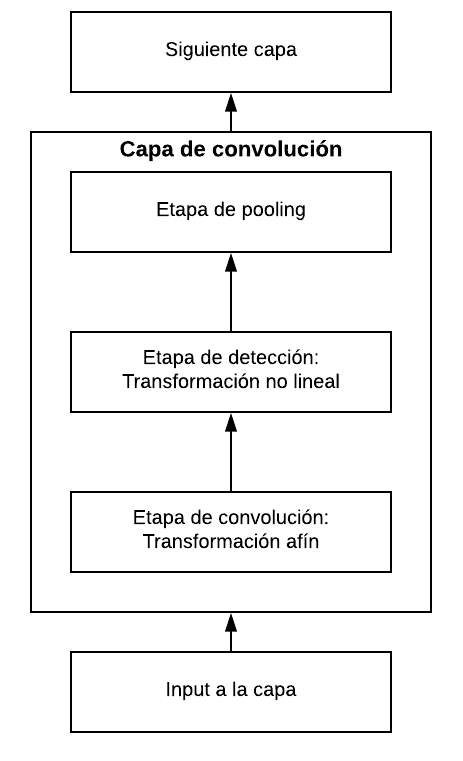
\includegraphics[scale=.8]{img/cap7_CNN.png}
\end{figure}

\textbf{Max pooling} retorna el valor m\'aximo de un output en una vecindad rectangular. Las operaciones de pooling permiten que la red sea invariante a peque{\~{n}}as transformaciones en el input. Pooling tambi\'en es escencial para procesar inputs de tama{\~{n}}o variable (por ejemplo im\'agenes de distinto tama{\~{n}}o).

Otras diferencias con respecto a la operaci\'on de convoluci\'on en el contexto de redes neuronales son, por ejemplo, el aplicar m\'ultiples convoluciones en paralelo, esto permite extraer distintos tipos de atributos en vez de 1 solo. Por otro lado, el \textbf{stride} hace referencia a cada cu\'antos pixeles se quieren convolucionar en cada direcci\'on en el output. En la figura se muestra el ejemplo de una convoluci\'on con stride. Esta operaci\'on permite reducir nuevamente el costo computacional. Esto tambi\'en implica que el output disminuye su tama{\~{n}}o en cada capa. El uso de \textit{padding} puede revertir esto. \textbf{Padding} se refiere a agrandar el input con ceros para hacerlo m\'as amplio. Una convoluci\'on en la que no se usa \textbf{zero-padding} se conoce como \textbf{valid}. Una convoluci\'on que mantiene el tama{\~{n}}o desde el input al output se conoce como \textbf{same} (ver figura). En la pr\'actica, las capas de una red convolucional usan operaciones entre una convoluci\'on valid y same.

\begin{figure}[H]
\captionsetup{font=small,labelfont=small}
\caption{Convoluci\'on con un stride igual a 2}
\centering
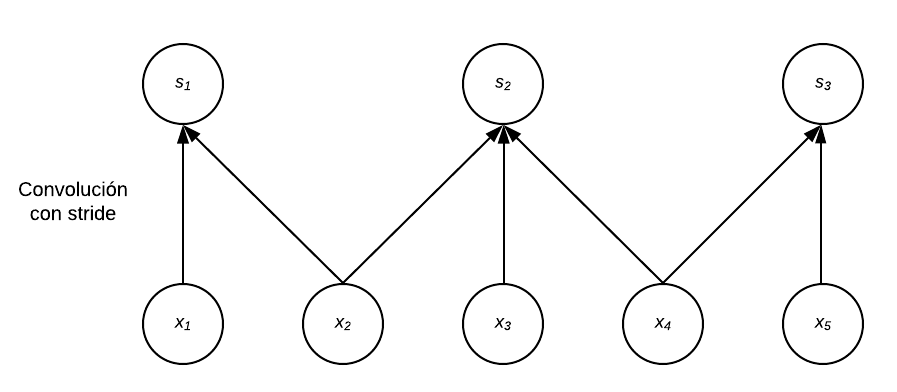
\includegraphics[scale=.8]{img/cap7_stride.png}
\end{figure}

\begin{figure}[H]
\captionsetup{font=small,labelfont=small}
\caption{Efecto de no usar zero-padding en una red convolucional (Arriba) y efecto de usar zero padding en una red convolucional (Abajo) en cuanto al tama{\~{n}}o de la red}
\centering
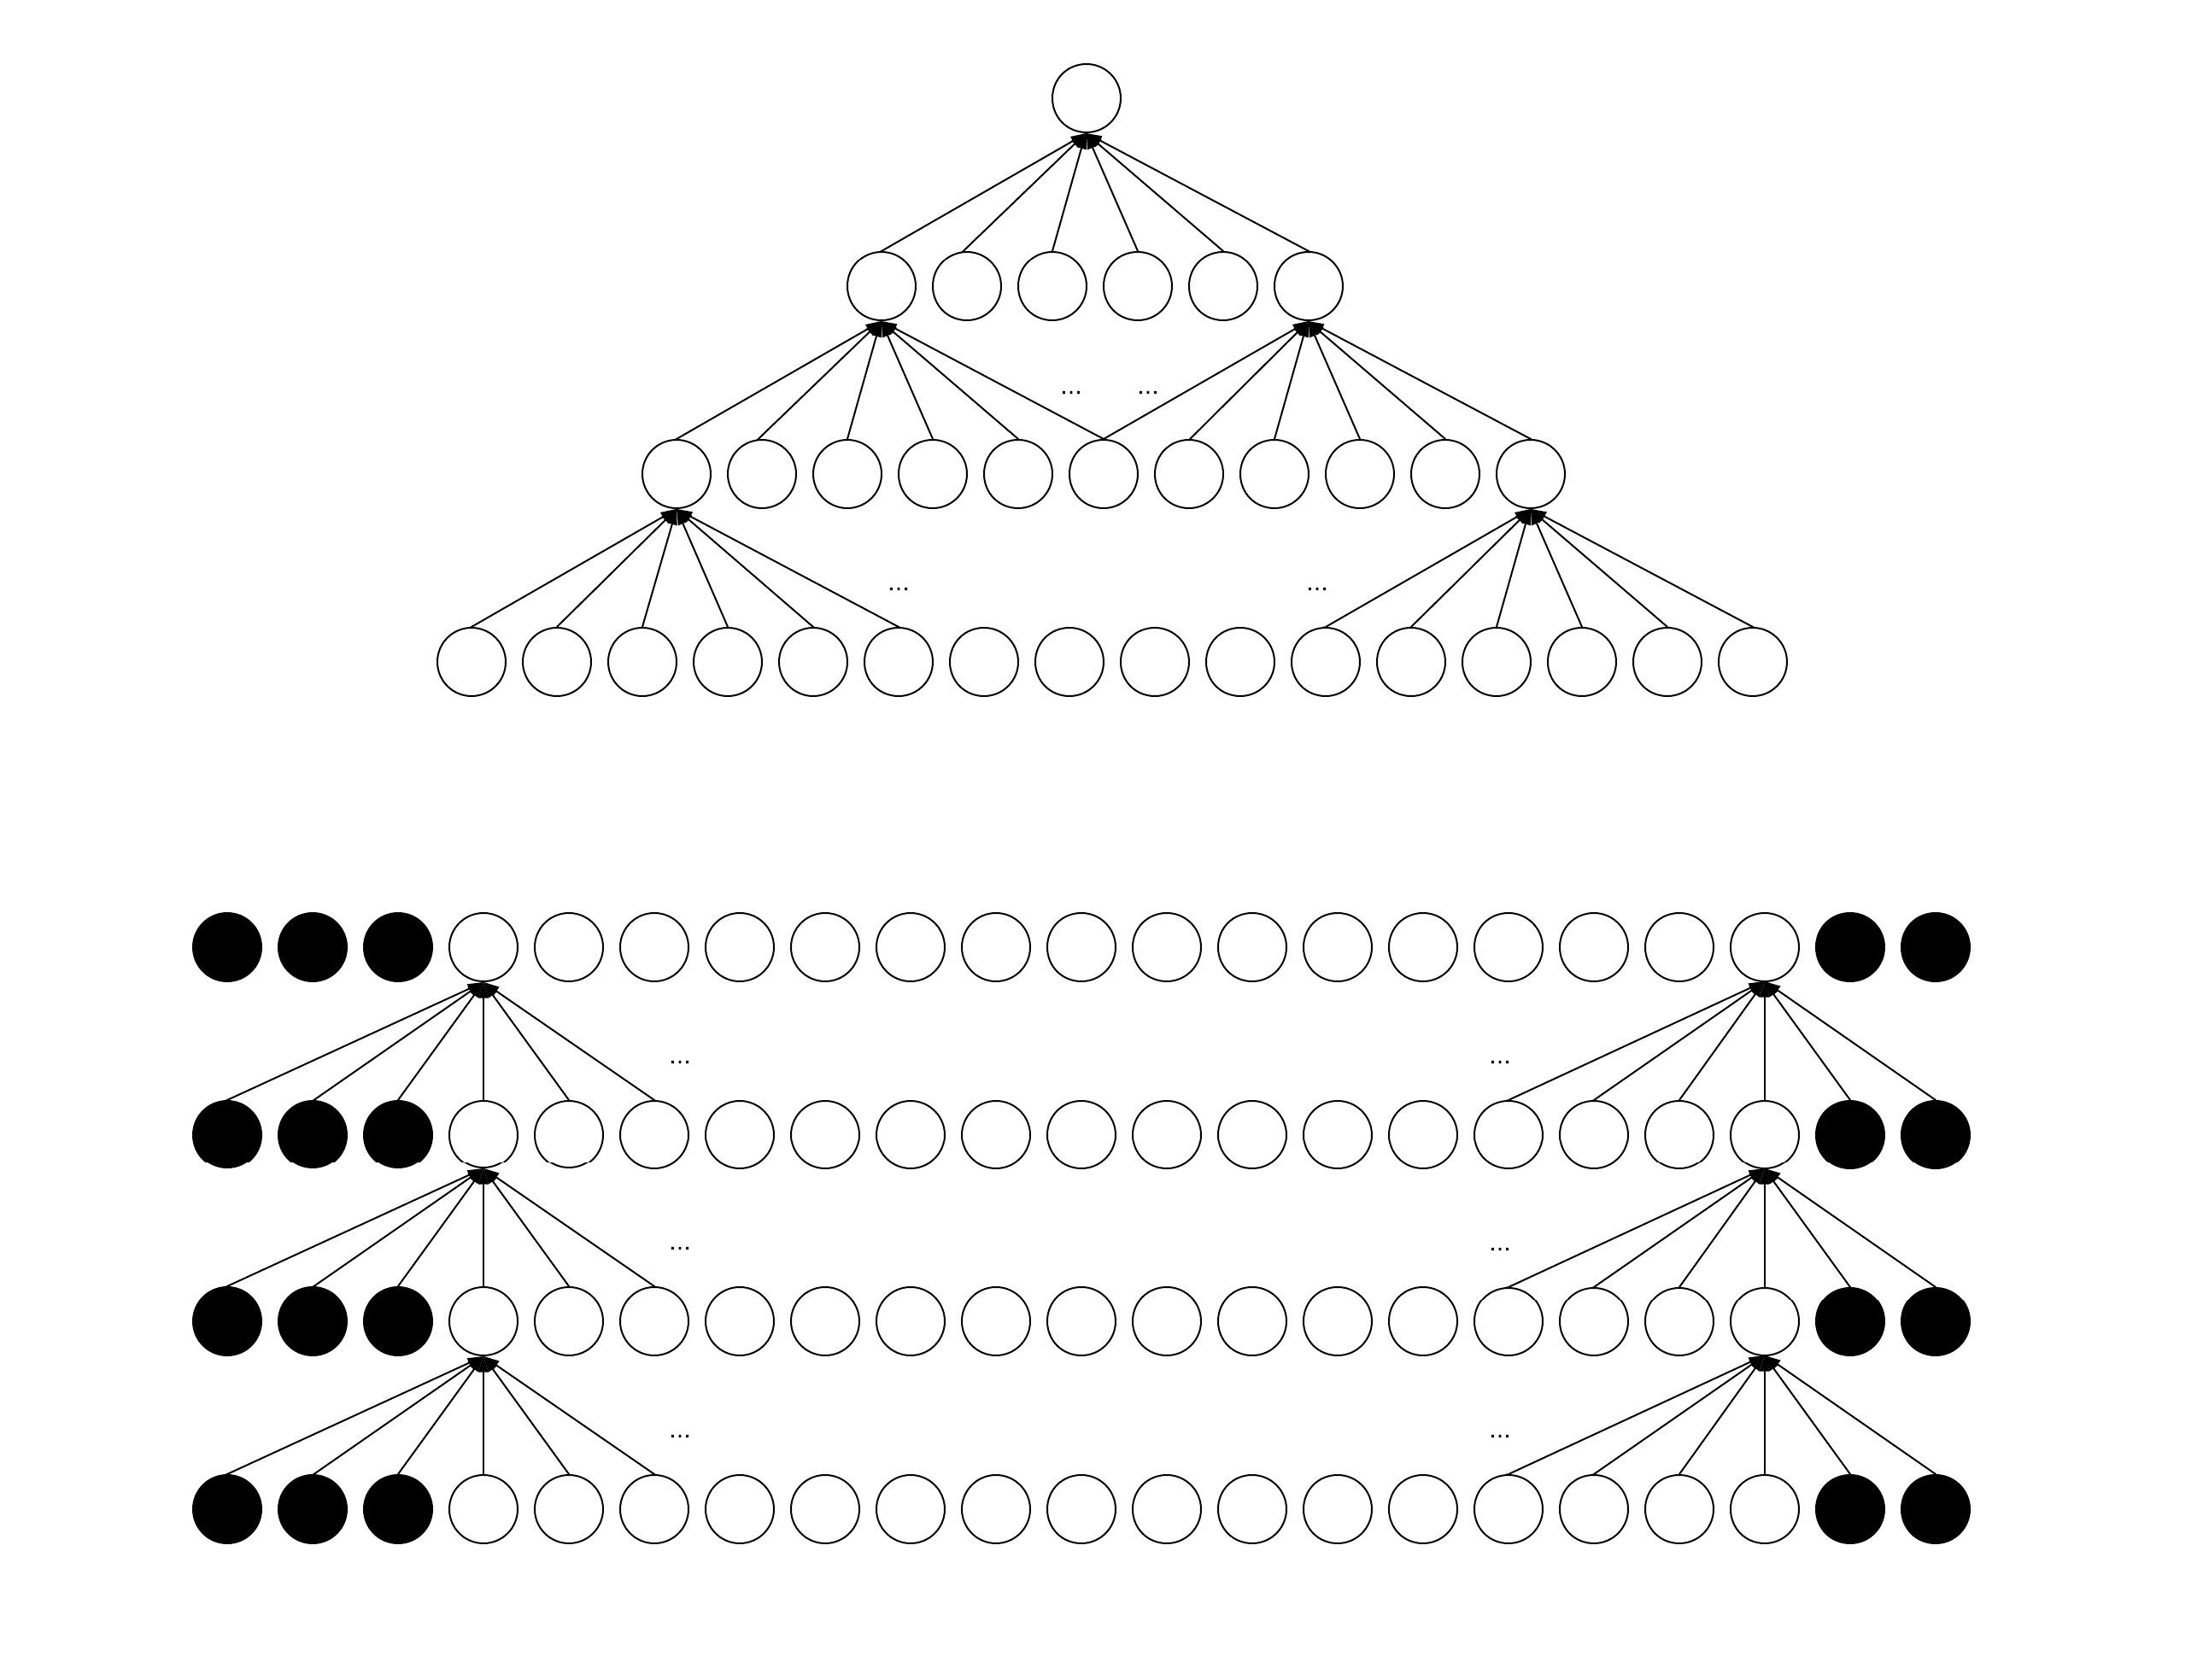
\includegraphics[scale=.15]{img/cap7_padding.png}
\end{figure}

\subsubsection{Redes neuronales recurrentes}

Las \textbf{redes neuronales recurrentes} o \textbf{RNNs} son una familia modelos de redes neuronales especializados para procesar datos secuenciales, $\bm{x}^{(1)},...,\bm{x}^{(\tau)}$. Las RNNs tambi\'en comparten par\'ametros, pero en una forma muy distinta que las CNNs. En una RNN, cada miembro del output en una etapa es una funci\'on de cada miembro del output de la etapa anterior.

Se denota por $\bm{h}^{(t)}$ al estado de un sistema din\'amico que involucra una recurrencia conducido por un input externo $\bm{x}^{(t)}$:

\begin{equation}
\bm{h}^{(t)} = f(\bm{h}^{(t-1)}; \bm{x}^{(t)}, \bm{\theta})
\end{equation}

La figura siguiente muestra una red recurrente que procesa un input $\bm{x}$ incorpor\'andolo al estado $\bm{h}$ que es traspasado a trav\'es del tiempo.

\begin{figure}[H]
\captionsetup{font=small,labelfont=small}
\caption{Ejemplo de una red recurrente sin output}
\centering
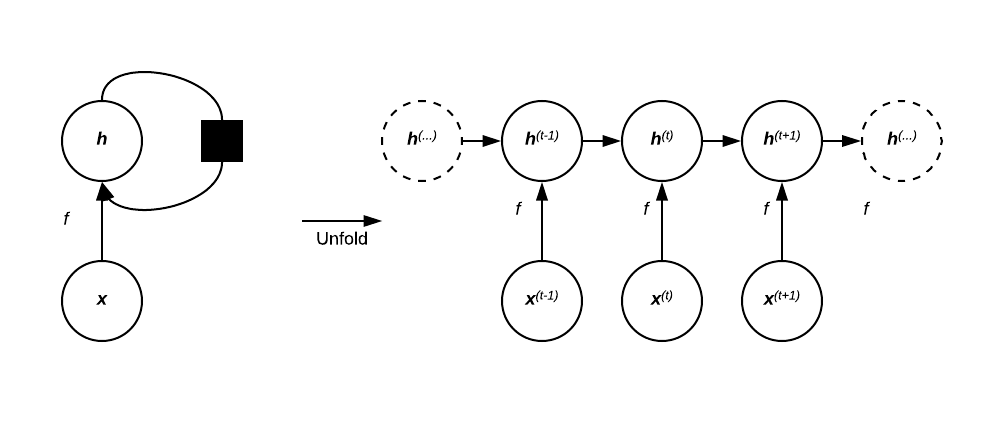
\includegraphics[scale=.5]{img/cap7_RNN1.png}
\end{figure}

Las redes recurrentes se pueden construir de muchas formas distintas. Al igual que una red neuronal puede representar casi cualquier funci\'on, una red recurrente modela cualquier funci\'on que involucre una recurrencia. Se puede representar el estado de una red recurrente luego de $t$ pasos mediante una funci\'on $g^{(t)}$:

\begin{equation}
\bm{h}^{(t)} = g^{(t)}(\bm{x}^{(t)},\bm{x}^{(t-1)},...,\bm{x}^{(1)}) =  f(\bm{h}^{(t-1)}; \bm{x}^{(t)}, \bm{\theta})
\end{equation}

Existen varios tipos de RNNs que se han dise{\~{n}}ado para distintos fines. Algunos ejemplos de estas son:

\begin{itemize}
  \item Redes recurrentes que producen un output en cada instante de tiempo y tienen conexiones entre todas las unidades escondidas
  \item Redes recurrentes que producen un output en cada instante de tiempo y tienen conexiones entre el output a la unidad escondida del siguiente instante
  \item Redes recurrentes con conexiones entre las unidad escondidas, que procesan una secuencia entera antes de producir el output
\end{itemize}

La figura muestra un ejemplo de la arquitectura para el primer caso.

\begin{figure}[H]
\captionsetup{font=small,labelfont=small}
\caption{Ejemplo de una red recurrente que produce un output en cada instante de tiempo, y que comparte el estado a trav\'es del tiempo}
\centering
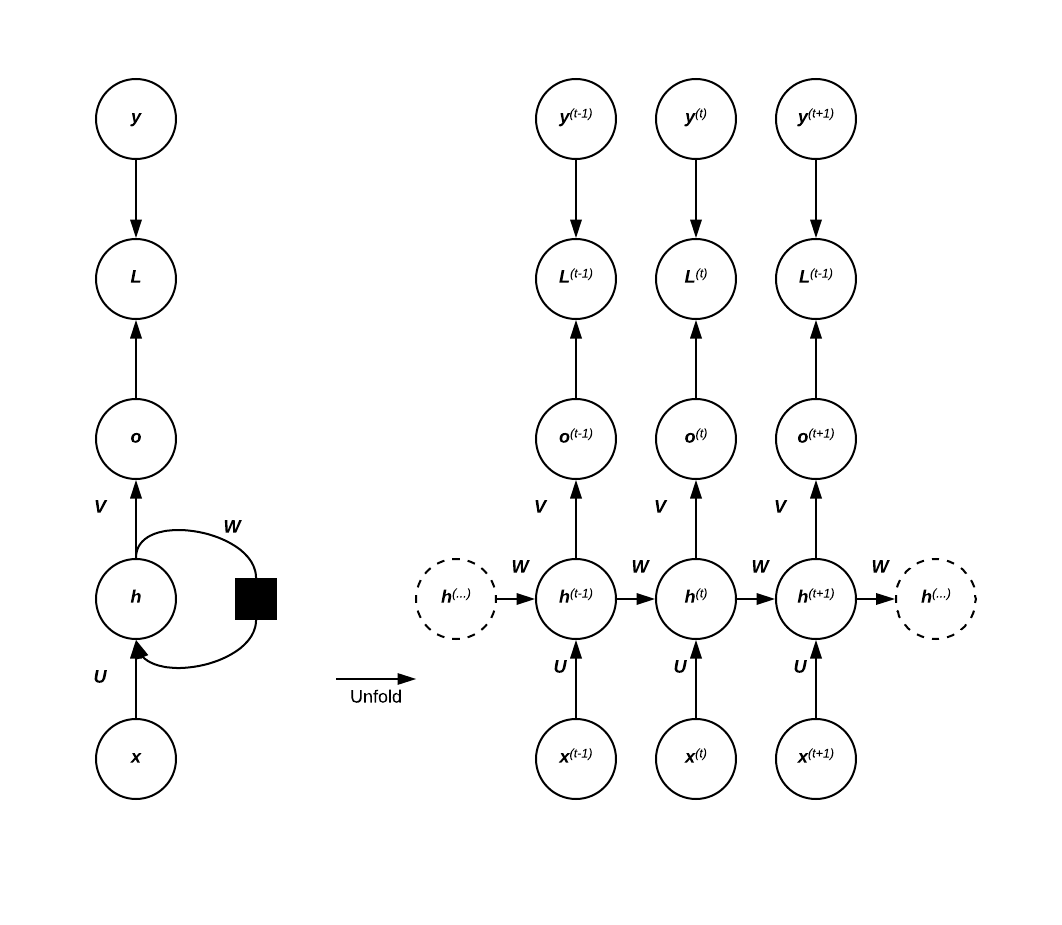
\includegraphics[scale=.5]{img/cap7_RNN2.png}
\end{figure}

Esta red presentada puede ser usada para producir palabras en cada instante, y as\'i producir oraciones que hagan sentido en una conversaci\'on. Como ejemplo de entrenamiento de una red con esta arquitectura, en donde en la \'ultima capa se decide mediante una funci\'on softmax la palabra m\'as probable que deba seguir a la palabra anterior, se tienen las ecuaciones de \textit{forward propagation} para cada instante de tiempo:

\begin{equation}
\begin{array}{l}
\bm{a}^{(t)} = \bm{b} + \bm{W}\bm{h}^{(t-1)}+\bm{U}\bm{x}^{(t-1)} \\
\bm{h}^{(t)} = \textrm{tanh}(\bm{a}^{(t)}) \\
\bm{o}^{(t)} = \bm{c} + \bm{V}\bm{h}^{(t)} \\
\hat{\bm{y}}^{(t)} = \textrm{softmax}(\bm{o}^{(t)})
\end{array}
\end{equation}

El algoritmo aplicado para obtener el gradiente en este tipo de arquitectura se conoce como \textbf{back-propagation through time}, y consiste en aplicar el algoritmo de \textit{back-propagation} generalizado para el grafo computacional \textit{unfolded} de la red, como los mostrados en las figuras de redes recurrentes.

Las redes recurrentes sufren de no poder recordar largas dependencias a trav\'es del tiempo, debido a que las recurrencias implican multiplicar una matriz de pesos m\'ultiples veces a trav\'es de la red, provocando superficies planas o muy empinadas que resultan en que los algoritmos de aprendizaje por gradiente tengan problemas de \textbf{vanishing gradients} o \textbf{exploding gradients}, respectivamente. Arquitecturas que han logrado superar esto son las que incluyen compuertas (funciones sigmoidales) que deciden autom\'aticamente qu\'e olvidar y qu\'e seguir propagando a trav\'es de la red. Estos son los modelos de \textbf{gated recurrent units} (\textbf{GRUs}) y \textbf{long-short term memory network} (\textbf{LSTM}).

\subsubsection{Autoencoders}

Un \textbf{autoencoder} es una red neuronal que busca replicar el input hacia el output, osea, se busca que la información que entra a la red sea lo más parecida posible a la de salida, para lo cual cuenta con una capa interna $\bm{h} = f(\bm{x})$ que codifica el input (genera una representaci\'on de este) llamada \textbf{encoder} y una funci\'on que produce la reconstrucci\'on $\bm{r} = g(\bm{h})$, el \textbf{decoder}. Un \textit{autoencoder} buscar\'a aprender los \textit{encoder} y \textit{decoder} tales que $g(f(\bm{x})) = \bm{x}$ para todo $\bm{x}$. Como el modelo est\'a forzado a aprender los atributos m\'as importantes para que pueda efectivamente reproducir el input en su output, este aprender\'a en general propiedades \'utiles de los datos de entrenamiento. Los \textit{autoencoders} modernos modelan mappings estoc\'asticos $p_{\textrm{encoder}}(\bm{h}|\bm{x})$ y $p_{\textrm{decoder}}(\bm{x}|\bm{h})$, en vez de funciones determin\'isticas. En la figura se muestra la arquitectura de un \textit{autoencoder}.

\begin{figure}[H]
\captionsetup{font=small,labelfont=small}
\caption{Estructura de un \textit{autoencoder} t\'ipico}
\centering
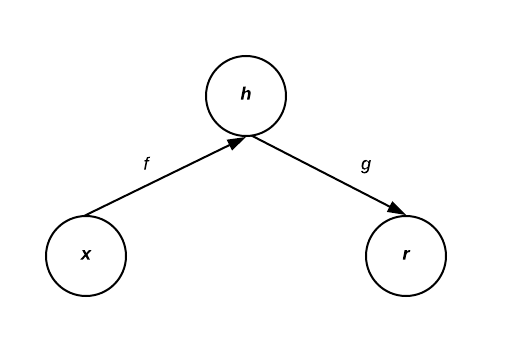
\includegraphics[scale=.8]{img/cap7_autoencoder.png}
\end{figure}

Una manera de obtener atributos \'utiles de $\bm{x}$ es forzando a que el \textit{encoder} tenga una dimensionalidad menor que el input. Este tipo de \textit{autoencoders} se denominan \textbf{undercomplete}. El aprendizaje se describe mediante la optimizaci\'on de la funci\'on de p\'erdida, $L(\bm{x}, g(f(\bm{x})))$. Cuando el \textit{decoder} es lineal y la funci\'on de p\'erdida es el error cuadr\'atico medio, un \textit{undercomplete autoencoder} aprende a generar el mismo subespacio que el algoritmo \textbf{principal component analysis} (\textbf{PCA}), es decir, el \textit{autoencoder} que fue entrenado para reproducir los datos de entrenamiento mediante una reducci\'on de dimensionalidad y una reconstrucci\'on aprendi\'o como efecto colateral el subespacio principal. Es as\'i como entonces, \textit{autoencoders} con \textit{encoders} y \textit{decoders} no lineales pueden aprender representaciones no lineales m\'as poderosas que PCA.

Un \textit{autoencoder} con dimensi\'on de su \textit{encoder} igual a la del input se conoce como \textbf{overcomplete}. Estos \textit{autoencoders}, al igual que los \textit{undercomplete}, pueden fallar en aprender una representaci\'on \'util del input si tienen mucha capacidad, por lo que ser\'a importante tambi\'en regularizar estas redes neuronales.

Otras aplicaciones de los autoencoders, aparte de aprender una reducci\'on de dimensionalidad, es aprender representaciones \'utiles que sirvan para un posterior modelo de redes neuronales (o, m\'as general, de aprendizaje de m\'aquinas). Por ejemplo, en vez de usar \textbf{one-hot-vectors} para representar palabras (en donde se tiene un vector del largo de cierto vocabulario compuesto por ceros excepto para la palabra que se quiere representar, indicando un valor de 1 en esa posici\'on), se pueden usar \textbf{embeddings}, que son representaciones del input a un espacio de valores reales. A diferencia de los \textit{one-hot-vectors}, en un \textit{embedding} la distancia entre las representaciones del texto s\'i tiene un significado, y este tipo de representaciones podr\'ia entregar mejores resultados en la tarea en que se est\'e usando.

\subsubsection{Redes generativas adversariales}

Una \textbf{red generativa adversarial} (o \textbf{GAN}) se basa en un escenario de teor\'ia de juegos, en donde una \textbf{red generadora} debe competir con un adversario. La red generadora produce muestras $\bm{x} = g(\bm{z};\bm{\theta}^{(g)})$, mientras que una \textbf{red discriminadora} trata de distinguir entre muestras obtenidas de los datos de entrenamiento y muestras generadas por la red generadora. El discriminador retorna una probabilidad, $d(\bm{x};\bm{\theta}^{(d)})$, indicando la probabilidad de que $\bm{x}$ sea un dato real y no uno simulado.

Para formular el aprendizaje, se describe un juego de suma cero en donde una funci\'on $v(\bm{\theta}^{(g)},\bm{\theta}^{(d)})$ determina el pago del discriminador, y el generador recibe $-v(\bm{\theta}^{(g)},\bm{\theta}^{(d)})$ como pago. As\'i, durante el entrenamiento cada jugador intenta maximizar su propio pago, para que en convergencia se tenga

\begin{equation}
g^{*} = \textrm{arg} \textrm{min}_{g} \textrm{max}_{d} v(g,d)
\end{equation}

Esto motiva a que el discriminador aprenda a clasificar correctamente entre muestras reales y falsas y, simulat\'aneamente, el generador intenta enga{\~{n}}ar al clasificador para que crea que las muestras generadas son reales. En convergencia, las muestras del generador son indistinguibles de los datos reales. Una motivaci\'on del uso de GANs es que cuando $\textrm{max}_{d} v(g,d)$ es convexa en $\bm{\theta}^{(g)}$, el procedimiento asegura la convergencia.

\begin{figure}[H]
\captionsetup{font=small,labelfont=small}
\caption{Im\'agenes generadas por una GAN entrenada con el set de datos LSUN. (Izquierda) Im\'agenes de dormitorios generadas por el modelo DCGAN (imagen de Radford et al., 2015). (Derecha) Im\'agenes de iglesias generadas por el modelo LAPGAN (imagen de Denton et al., 2015)}
\centering
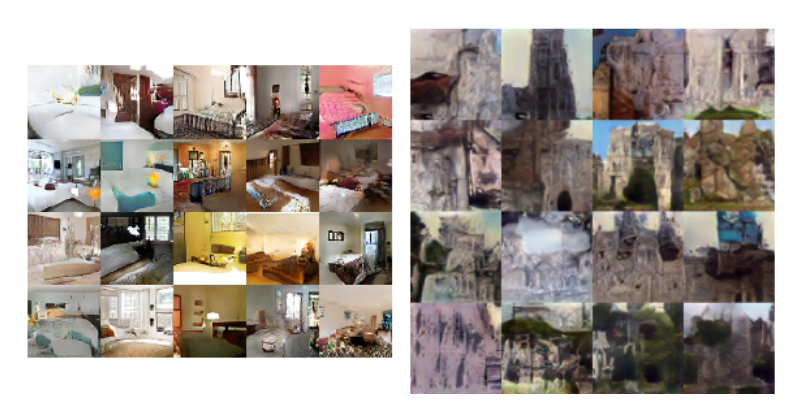
\includegraphics[scale=.75]{img/cap7_gans.PNG}
\end{figure}






























